\chapter{Testy i analiza wyników}
\vspace{-25pt}
\section{ Opis przeprowadzonych testów funkcjonalnych systemu}
Testom podlegać będzie wyjściowa ścieżka audio powstająca w wyniku działania algorytmu analizującego widmo piosenki wejściowej. Wyjściowa ścieżka audio będzie porównywana z wejściową piosenką według wybranych kryteriów sprawdzających jakość uzyskanej piosenki:\\
• poprawność rozpoznanych tonów,\\
• czas rozpoczęcia i zakończenia znajdowanych tonów,\\
• czy wszystkie wyszukane tony występują w wejściowym utworze.

Algorytmy analizy dźwięku zostały sprawdzone na trzech przykładowych piosenkach, które w oryginale głównie składają się z gry na instrumencie klawiszowym oraz wokalu:\\
• A Great Big World - Say Something \cite{say_something},\\
• Leonard Cohen - Hallelujah \cite{hallelujah},\\
• Michael Schulte - Falling Apart \cite{falling_apart}.

Następnie każda z nich została poddana testom w trzech różnych wersjach:\\
• piosenki powstałej z syntezy pliku z formatu midi na format wav,\\
• piosenki zagranej na instrumencie klawiszowym typu pianino, bądź fortepian \cite{say_something_piano_cover}\cite{hallelujah_piano_cover}\cite{falling_apart_piano_cover},\\
• oryginalnej piosenki wraz z wokalem.

Każda z powyższych wersji została sprawdzona przez trzy metody wyliczania progu detekcji. Poza algorytmem detekcji dźwięku testom podlega również wyświetlanie synthesii.

\newpage
\section{Testy}

\subsection{Pierwsza metoda detekcji głównych składowych utworu}

Metoda polegająca na wyznaczeniu progu granicznego z użyciem maksymalnej wartości amplitudy pomnożonej przez współczynnik m wyznaczony na podstawie wykresu. Dobierając odpowiednie wartości parametrów do wyznaczania wartości granicznej amplitudy najlepsze efekty dawała metoda łokciowa, która polegała na znalezieniu zgięcia odpowiadającemu nagłemu braku spadku ilości znajdowanych przez algorytm tonów. Dobrze jest to widoczne na syntetycznie stworzonej ścieżce dźwiękowej widocznej w środkowej kolumnie wykresu, gdzie każdy główny dźwięk ma małe oscylacje amplitudy.

\begin{figure}[h]
  \centering
  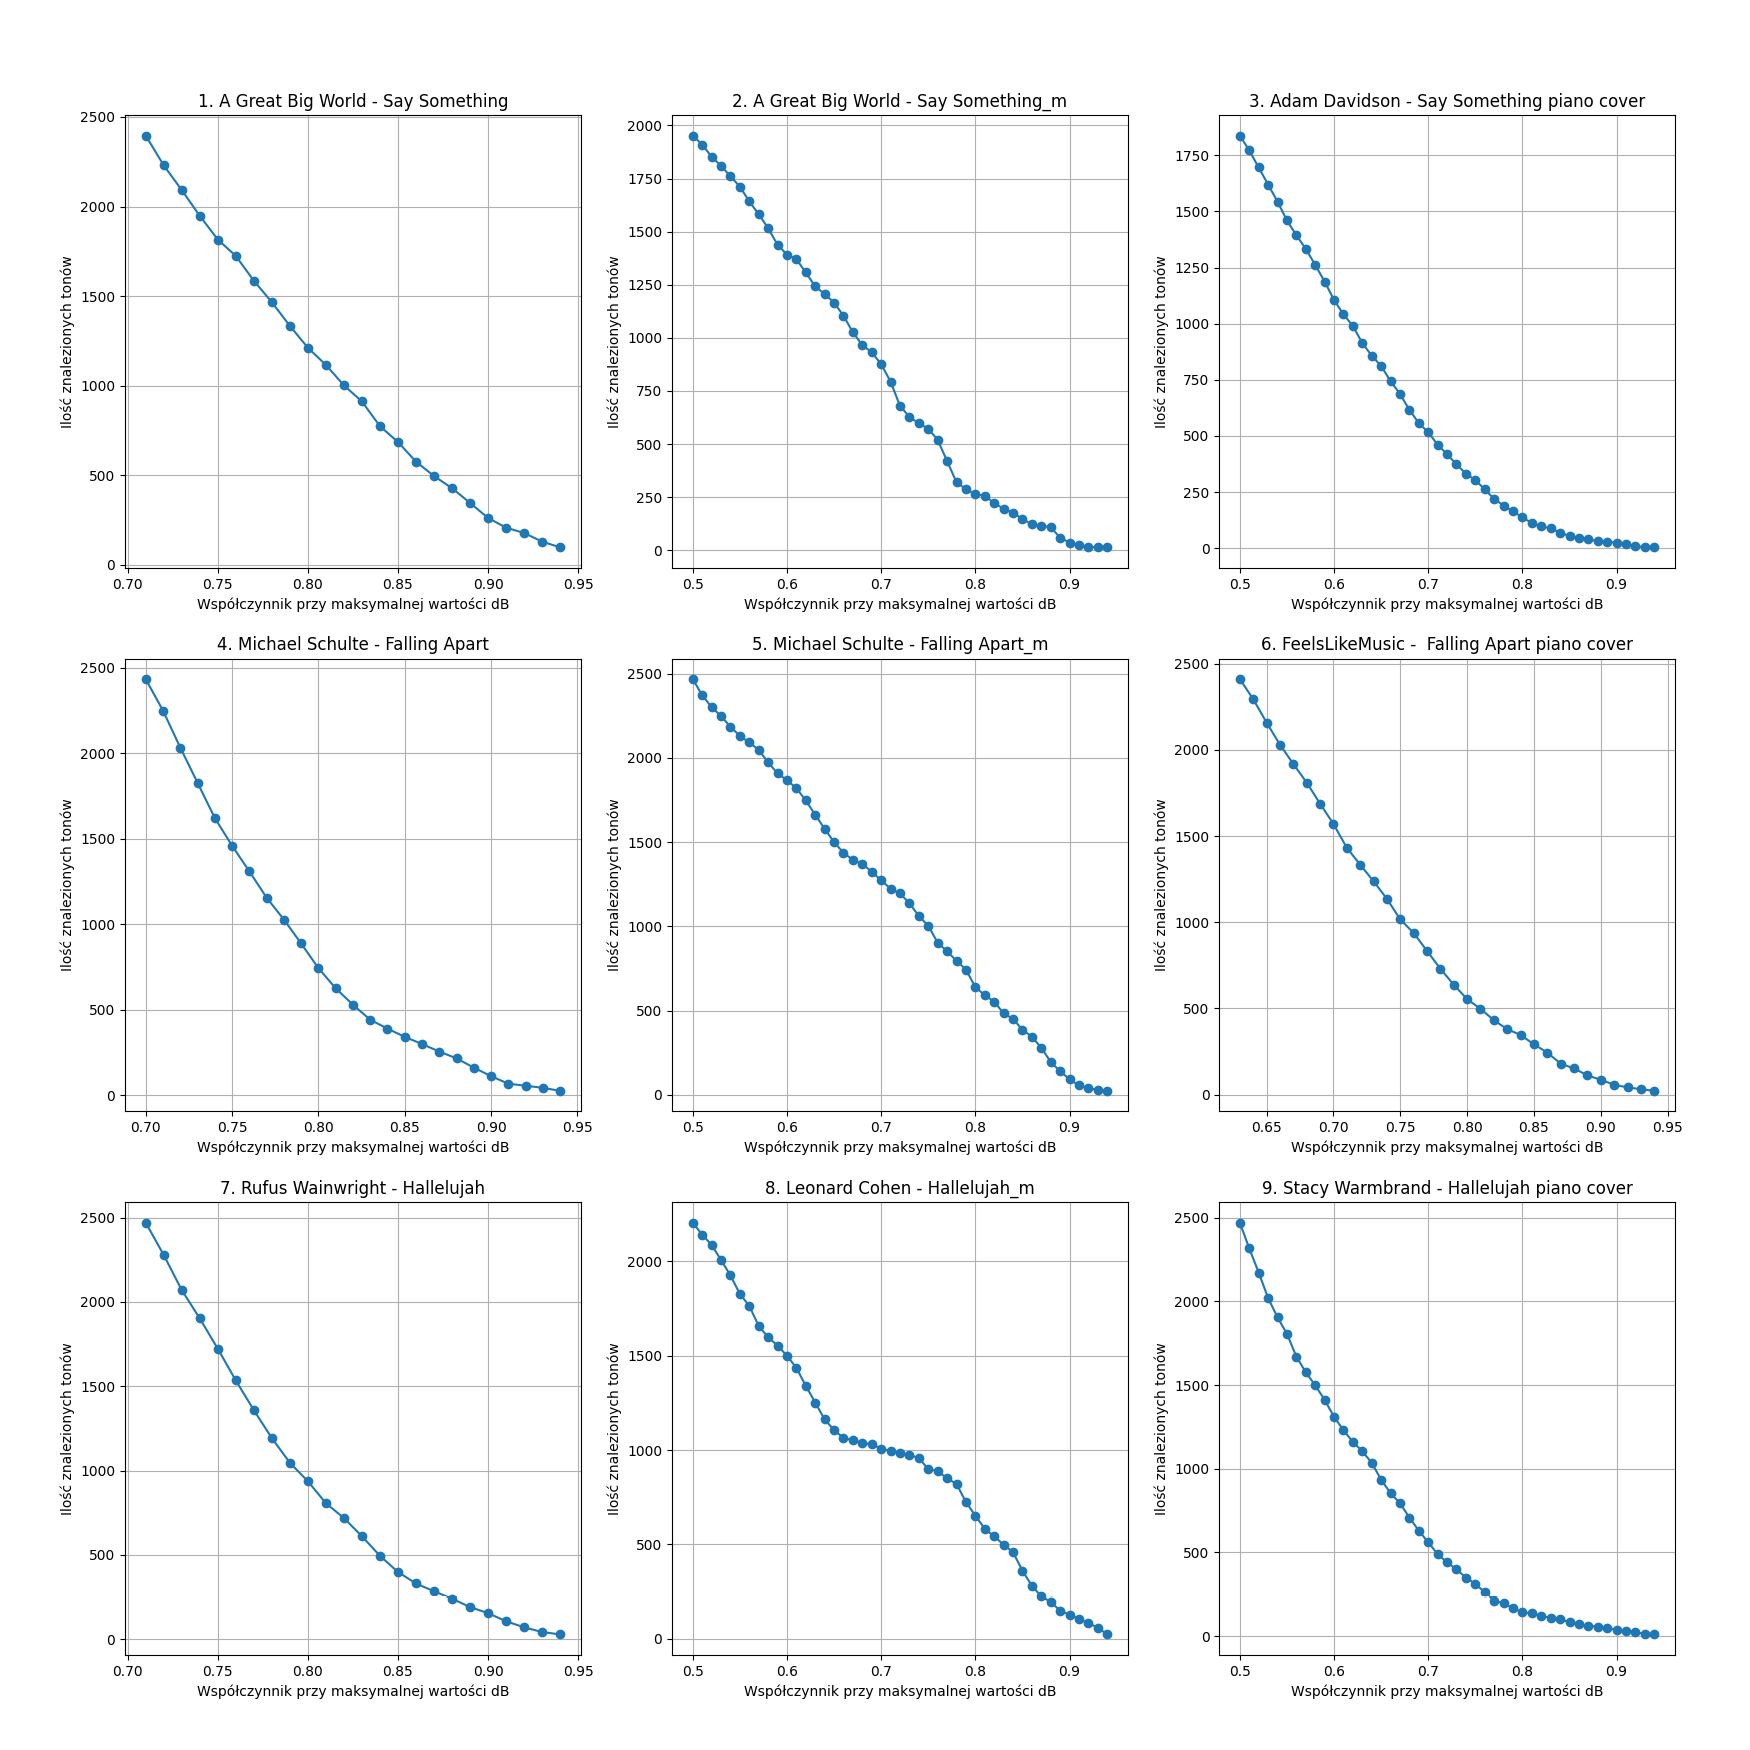
\includegraphics[width=0.94\textwidth]{img/5/wyk1.png}
  \caption{Wykres przedstawiający ilość wykrywanych tonów w metodzie pierwszej względem parametru m}
\end{figure}

Użycie tej metody dało bardzo dobre efekty przy utworze muzycznym stworzonym syntetycznie. Wykrywał składowe harmoniczne zrównujące się, bądź przewyższające amplitudę głównych dźwięków. Wyjściowa sekwencja z jednorazowo pomijanymi głównymi tonami oraz dodanymi przy błędnej identyfikacji dźwięków harmonicznych brzmiała identycznie jak wejściowa ścieżka audio. 

Przy utworze zagranym na pianinie nastąpił podział ze względu na zróżnicowanie amplitudowe wszystkich dźwięków. W bardziej wyciszonych fragmentach utworu metoda ta wykrywała pojedyncze dźwięki, bądź żadnych, natomiast we wzmocnionych momentach algorytm wykrywał zbyt wiele tonów wyłapując dźwięki harmoniczne oraz większe szumy, gdzie wyjściowa ścieżka dźwiękowa brzmiała podobnie do wejściowego utworu, jednakże przykryty wieloma źle zidentyfikowanymi dźwiękami. Jednakże fragmentami, gdzie każdy klawisz był grany z względnie równomierną siłą ścieżka wyjściowa brzmiała bardzo podobnie do piosenki poddanej analizie.
Przy analizie oryginalnego utworu, nastąpiły podobne problemy jak w analizie utworu granego na pianinie, jednakże dodatkowo powstały błędy w poprawności detekcji tonów w miejscach, gdzie przeplatały się dźwięki pianina oraz wokalu przez co powstawały dodatkowe luki w wynikowej sekwencji.

\subsection{Druga metoda detekcji głównych składowych utworu}

Metoda polegająca na wyznaczeniu progu granicznego z użyciem średniej ze wszystkich częstotliwości w małym przedziale czasu oraz maksymalnej wartości amplitudy. Współczynnik k oznaczał wartość, przez którą jest mnożona średnia oraz wchodził w skład wartości 1-k, przez którą mnożona jest maksymalna amplituda. Składowe następnie są sumowane i dzielone przez współczynnik d. Metoda ta jest wymaga przetwarzania znacznie więcej danych przez co jest zauważalnie wolniejsza niż pierwsza metoda.

W syntetycznych piosenkach metoda ta dała bardzo dobre efekty, ścieżka wyjściowa brzmiała również identycznie do wejściowej z pojedynczymi odchyłami, które lekko różniły się od poprzedniej metody w zależności od charakterystyki analizowanej piosenki.

Analiza gry na pianinie została poprawiona. Różnica pomiędzy fragmentami ścieżki audio została pomniejszona i detekcja stała się bardziej zbliżona do detekcji syntezowanej ścieżki dźwiękowej, niemniej jednak różnica nadal była widoczna.

Problem przy przetwarzaniu oryginalnego utworu pozostał nadal, pomimo poprawienia detekcji ogólnej. W konkretnych miejscach niejednokrotnie wykryte pianino zakrywało wokal, bądź odwrotnie w zależności od charakterystyki utworu.\\\\\\

\begin{figure}[h]
  \centering
  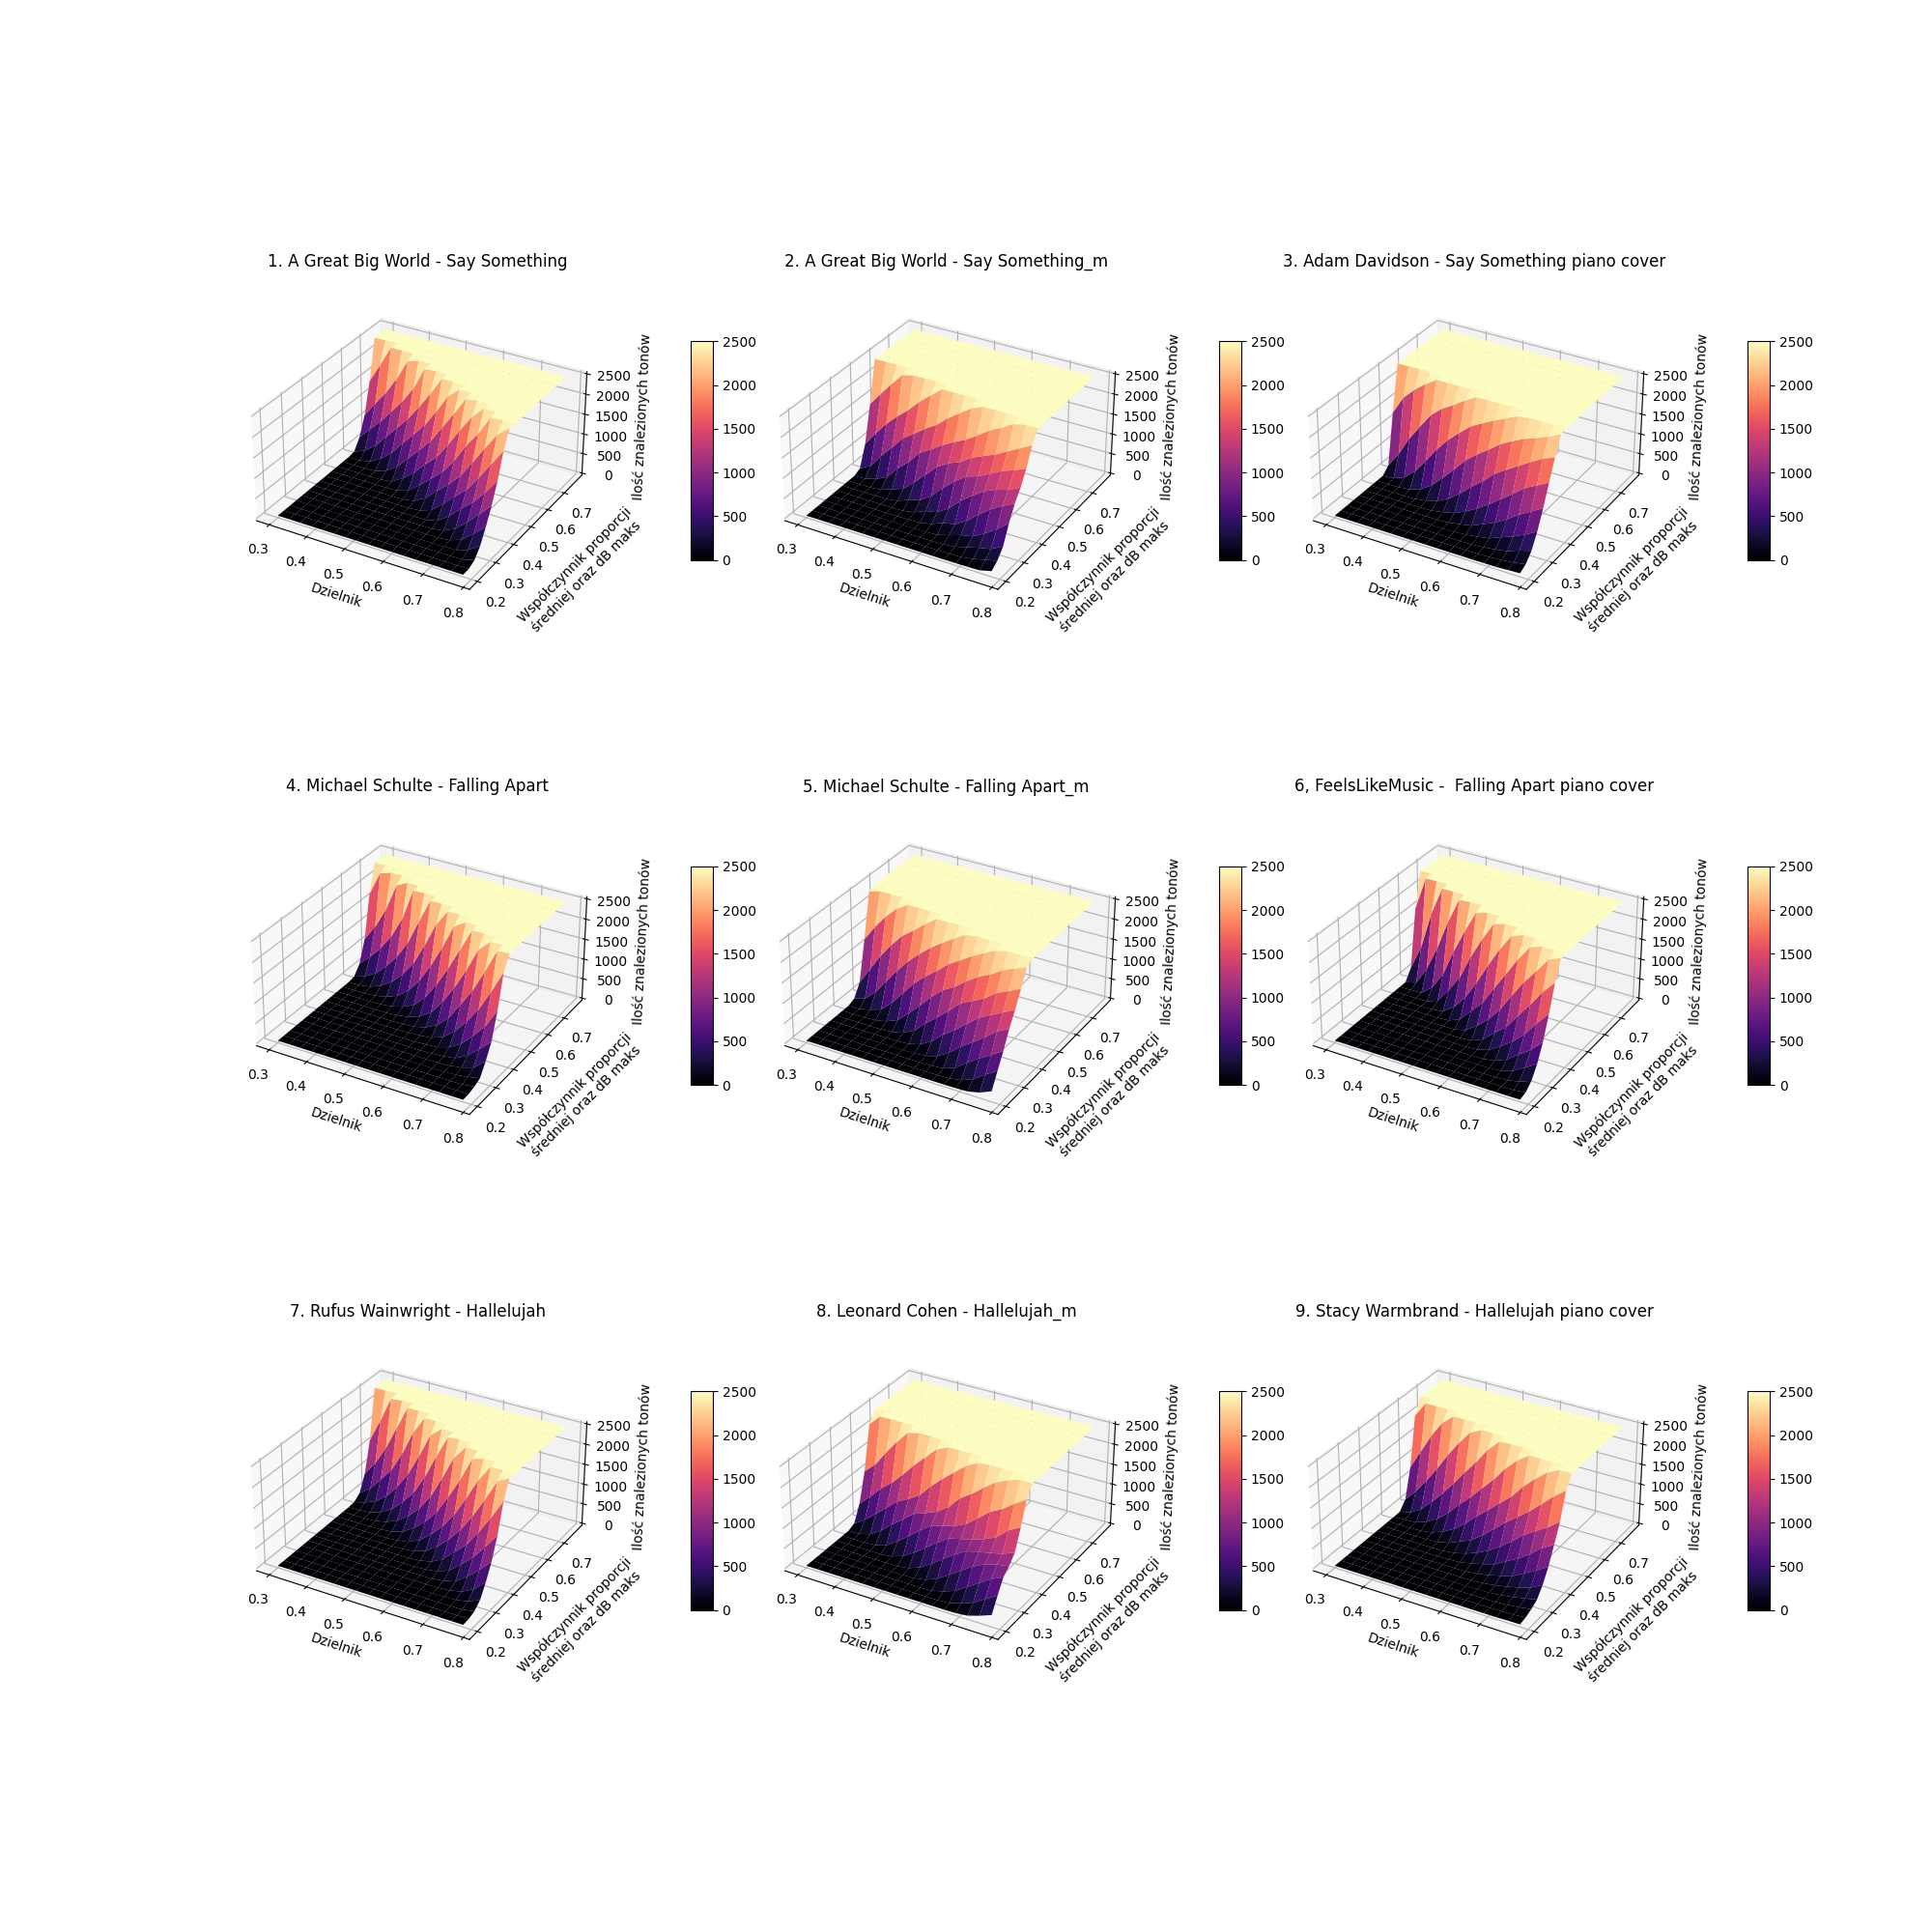
\includegraphics[width=0.94\textwidth]{img/5/wyk2.png}
  \caption{Wykres przedstawiający ilość wykrywanych tonów w metodzie drugiej względem parametrów k i d}
\end{figure}

\subsection{Trzecia metoda detekcji głównych składowych utworu}

Metoda polegająca na wyznaczeniu progu granicznego z użyciem maksymalnej wartości amplitudy oraz średniej ze wszystkich częstotliwości w małym przedziale czasu i małym przedziale częstotliwości. Współczynnik k oznaczał wartość, przez którą jest mnożona średnia oraz wchodził w skład wartości 1-k, przez którą mnożona jest maksymalna amplituda. Składowe następnie są sumowane i dzielone przez współczynnik d.

W syntetycznych piosenkach metoda ta dała również dobre efekty, jednakże identyfikując błędnie więcej składowych harmonicznych.\\

Analiza gry na pianinie została poprawiona. Różnica pomiędzy fragmentami ścieżki audio została jeszcze bardziej pomniejszona, jednak również wyłapując błędnie zauważalnie więcej składowych harmonicznych. Przetwarzanie oryginalnego utworu zostało nieznacznie poprawione, niestety kosztem uchwycenia niepożądanych częstotliwości.

\begin{figure}[h]
  \centering
  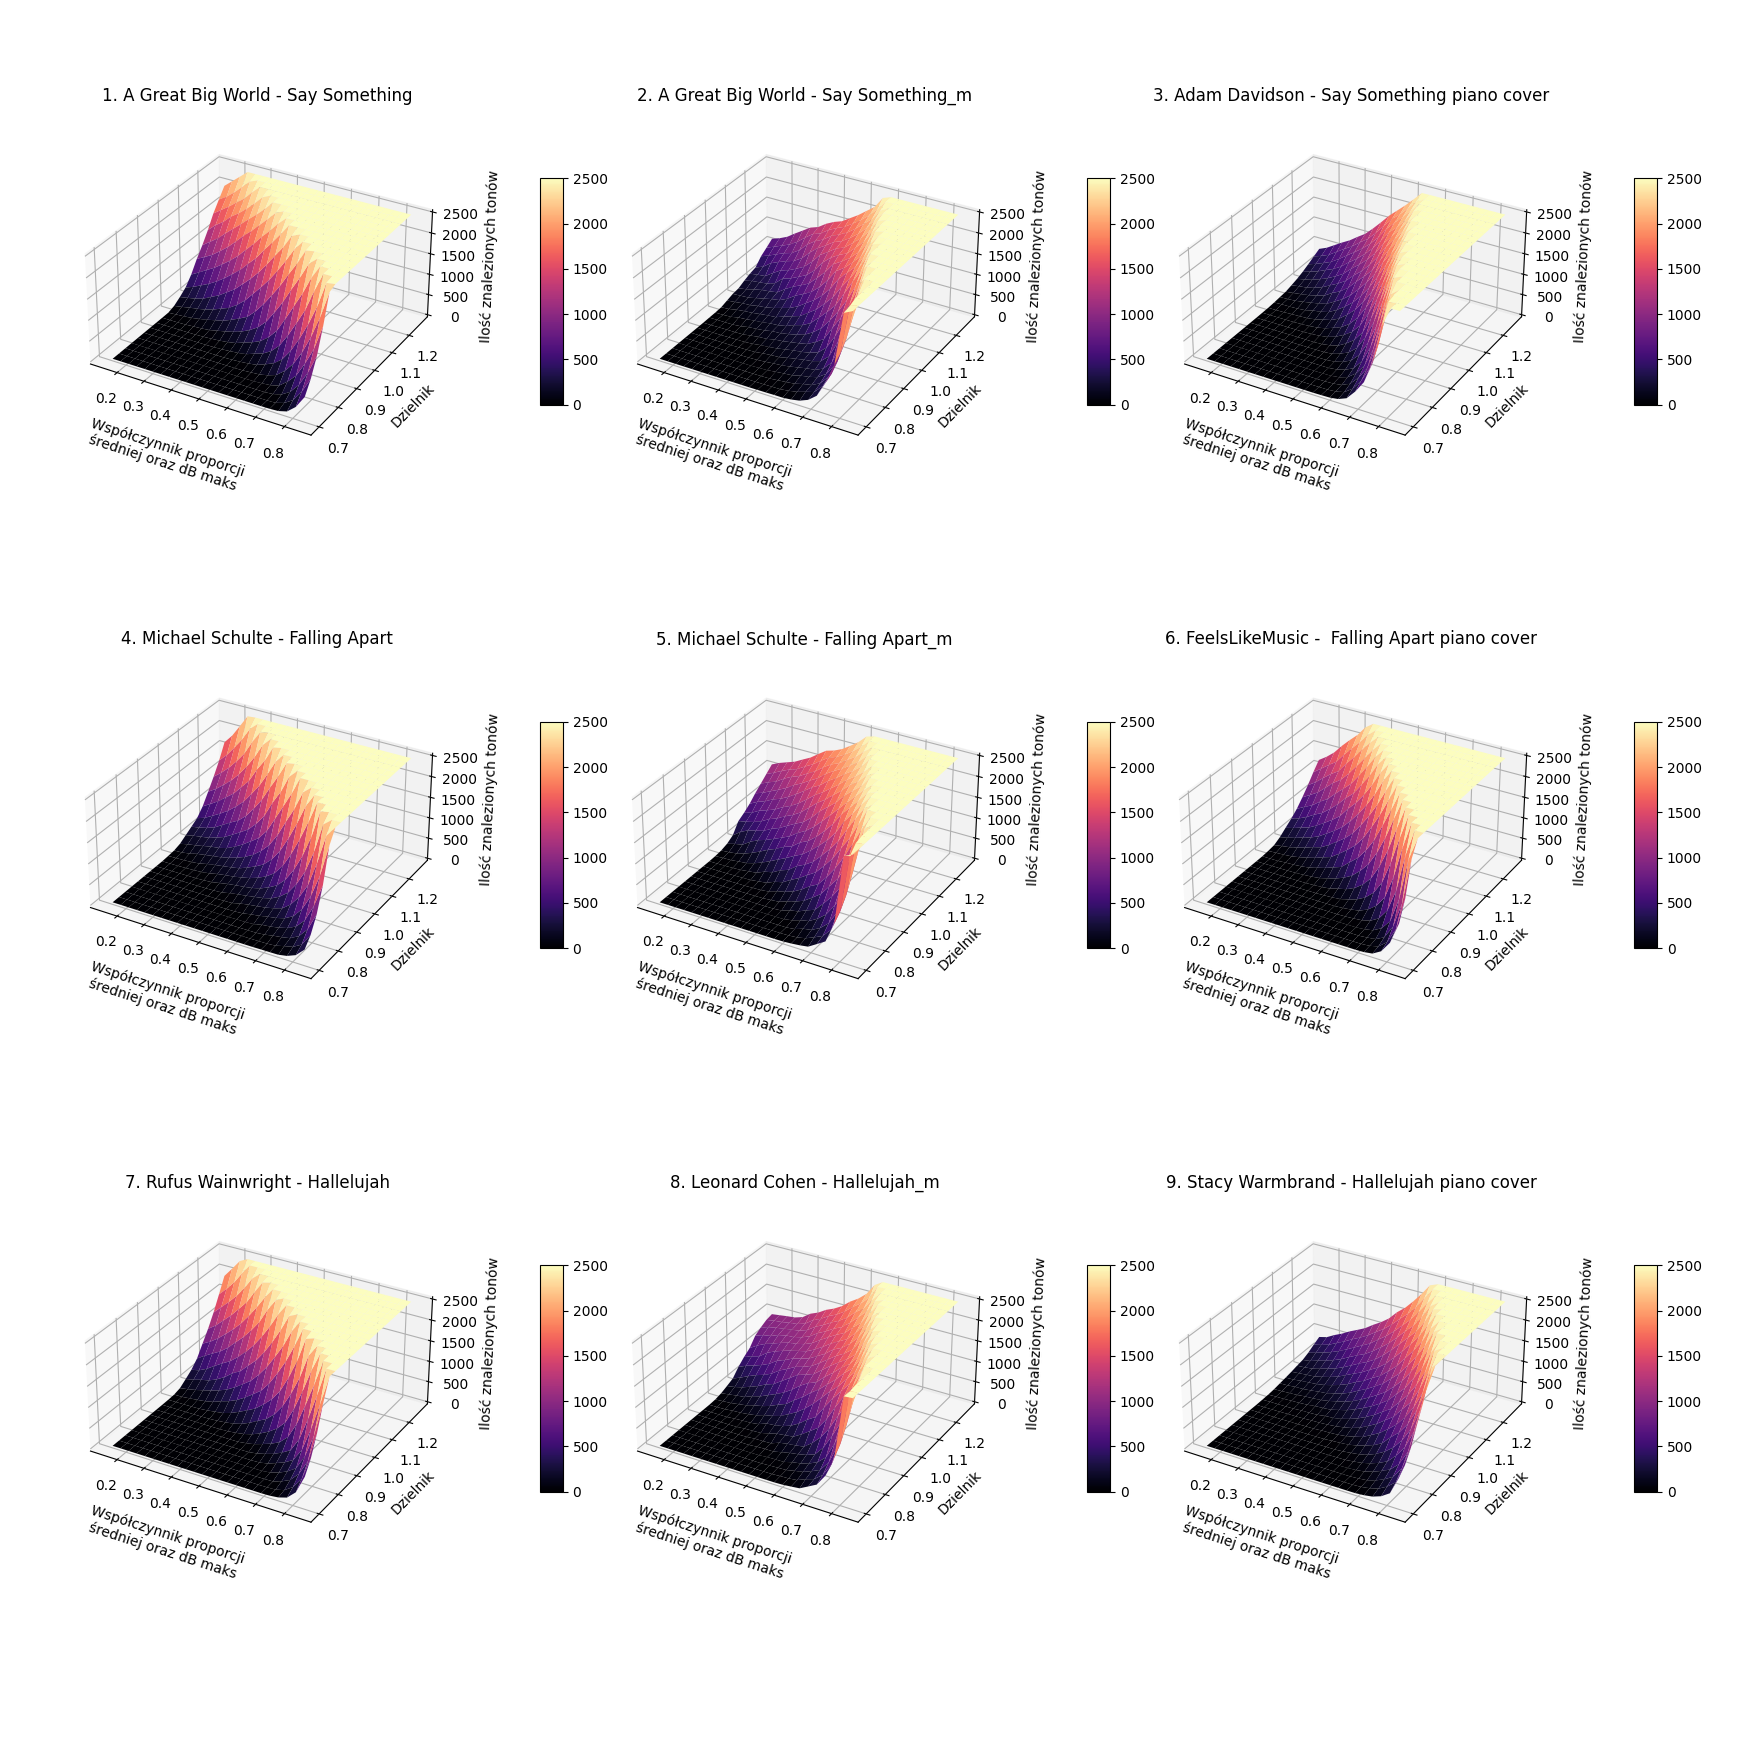
\includegraphics[width=0.94\textwidth]{img/5/wyk3.png}
  \caption{Wykres przedstawiający ilość wykrywanych tonów w metodzie trzeciej względem parametrów k i d}
\end{figure}

\newpage
\subsection{Say Something}

\textbf{Piosenka powstała z syntezy pliku midi}

\begin{figure}[h]
  \centering
  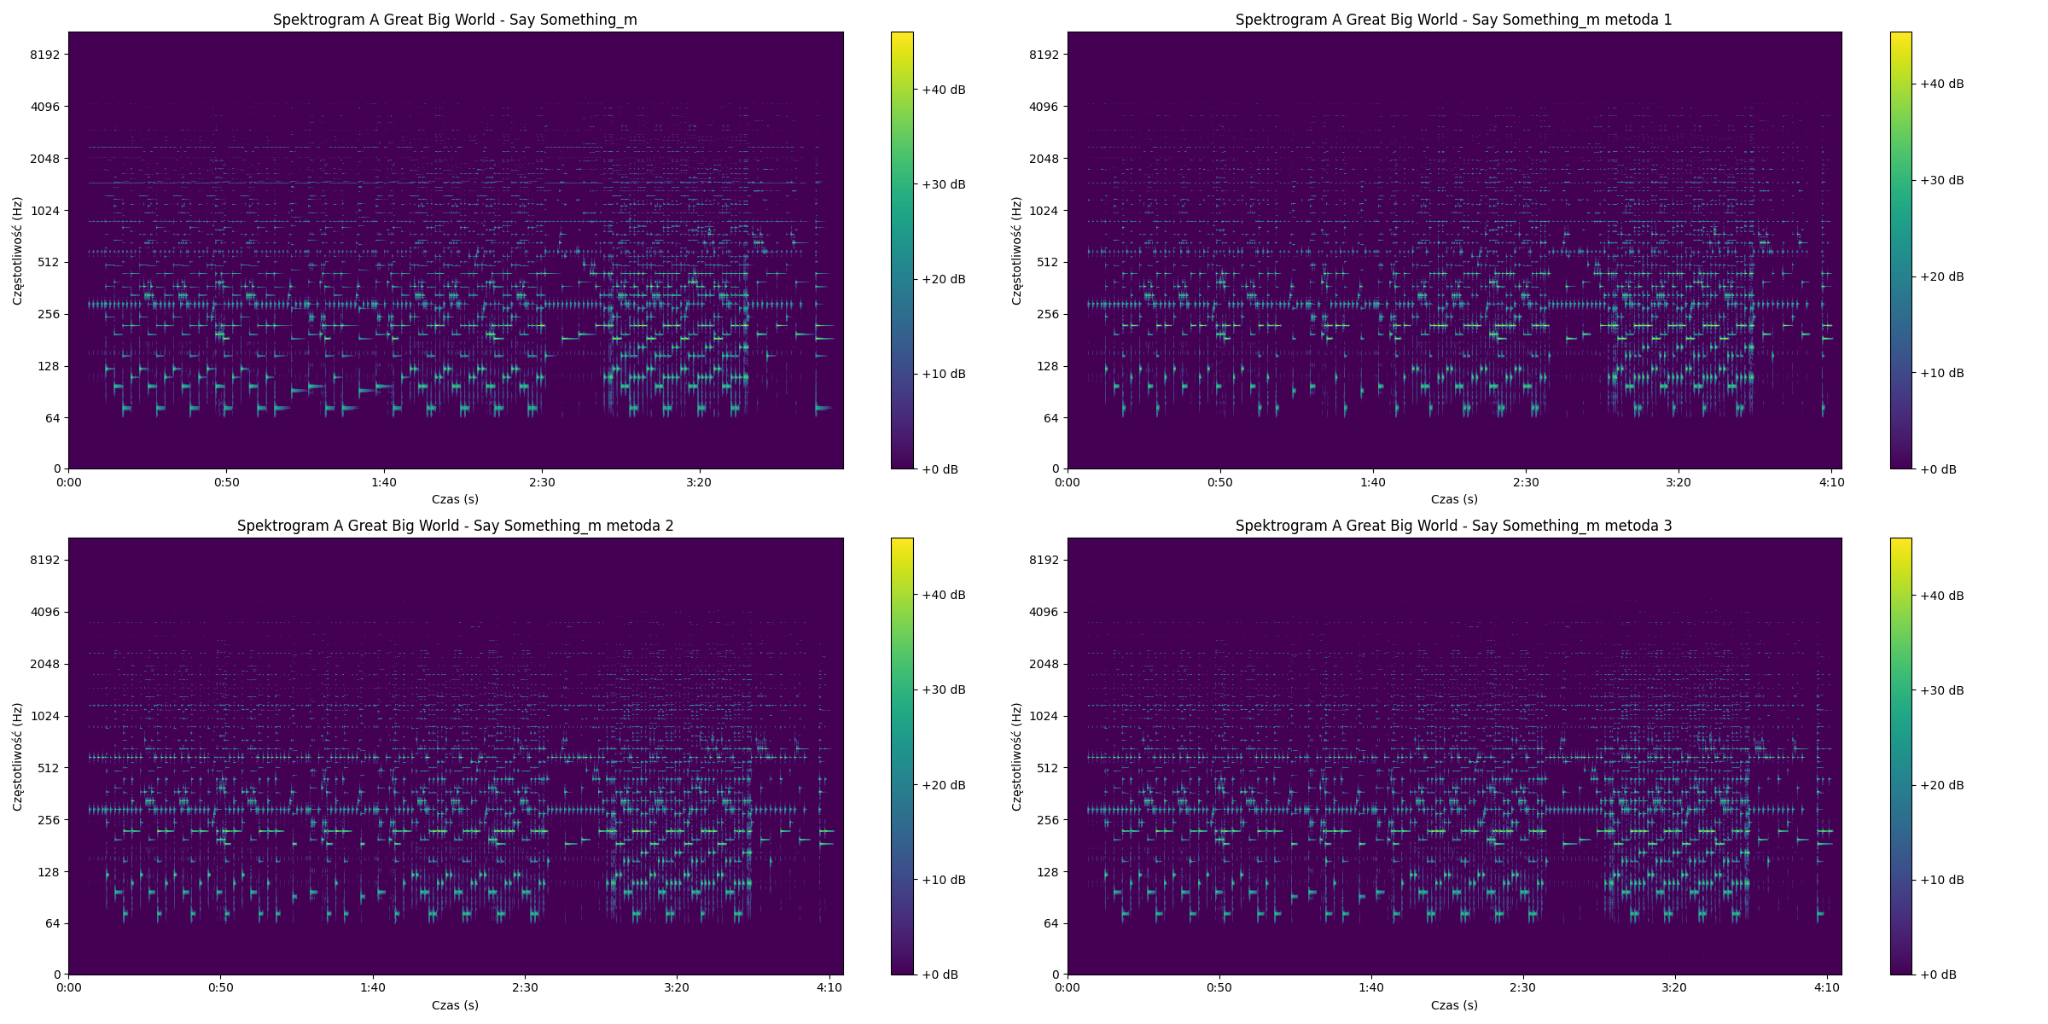
\includegraphics[width=0.82\textwidth]{img/5/wid1.png}
  \caption{Wykres przedstawiający widmo wejściowego nagrania oraz \\wyjściowych ścieżek dźwiękowych}
\end{figure}

\noindent Współczynnik m przy wartości maksymalnej użyty w pierwszej metodzie wynosił 0.66.
W drugiej metodzie współczynnik k, czyli stosunku średniej wszystkich wartości w małym otoczeniu czasu do wartości maksymalnej wynosił 0.4, a dzielnik d wynosił 0.6.
W trzeciej metodzie współczynnik k, czyli stosunku średniej wartości w małym otoczeniu do wartości maksymalnej wynosił 0.4, a dzielnik d wynosił 1.2.\\

\textbf{Piosenka zagrana na instrumencie klawiszowym typu pianino, bądź fortepian}

\begin{figure}[h]
  \centering
  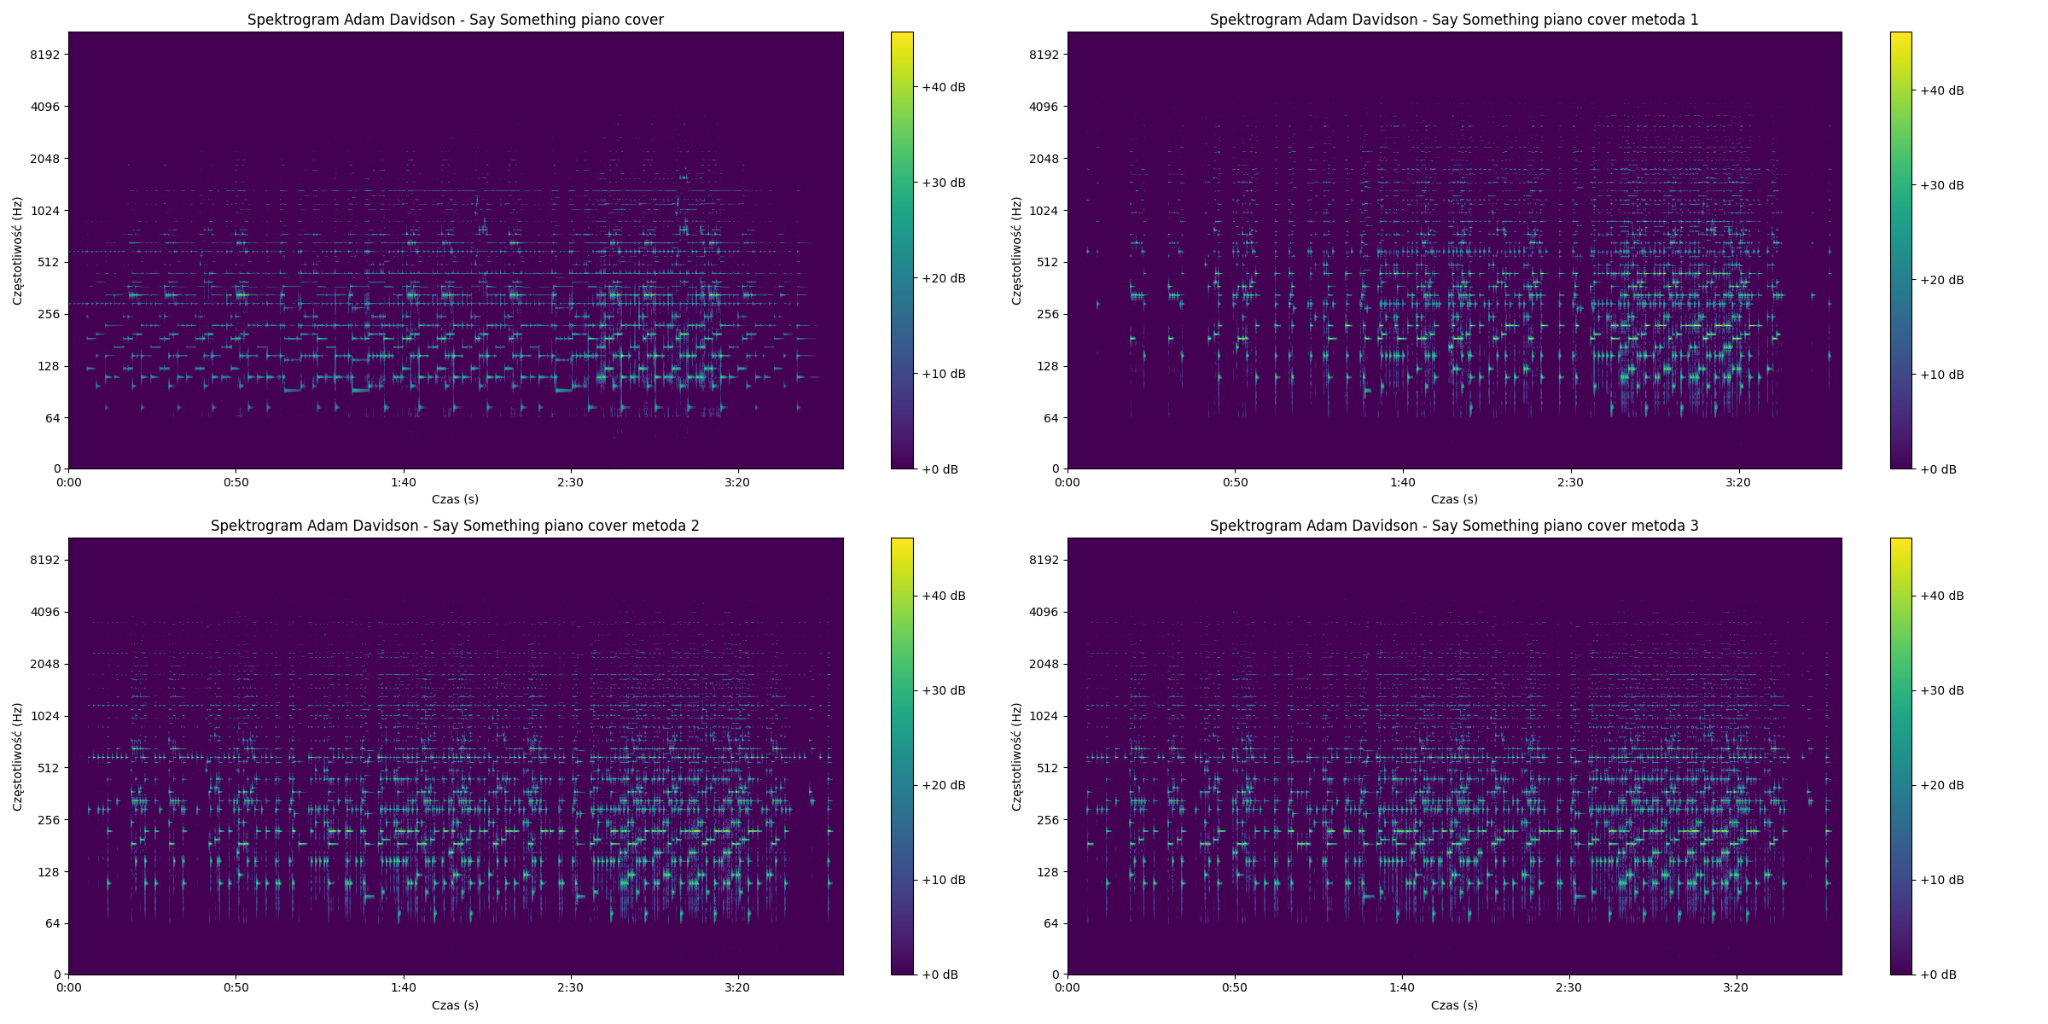
\includegraphics[width=0.82\textwidth]{img/5/wid2.png}
  \caption{Wykres przedstawiający widmo wejściowego nagrania oraz \\wyjściowych ścieżek dźwiękowych}
\end{figure}


\noindent Współczynnik m przy wartości maksymalnej użyty w pierwszej metodzie wynosił 0.62.
W drugiej metodzie współczynnik k, czyli stosunku średniej wszystkich wartości w małym otoczeniu czasu do wartości maksymalnej wynosił 0.4, a dzielnik d wynosił 0.6.
W trzeciej metodzie współczynnik k, czyli stosunku średniej wartości w małym otoczeniu do wartości maksymalnej wynosił 0.6, a dzielnik d wynosił 1.\\

\textbf{Oryginalna piosenka zawierająca wokal}

\begin{figure}[h]
  \centering
  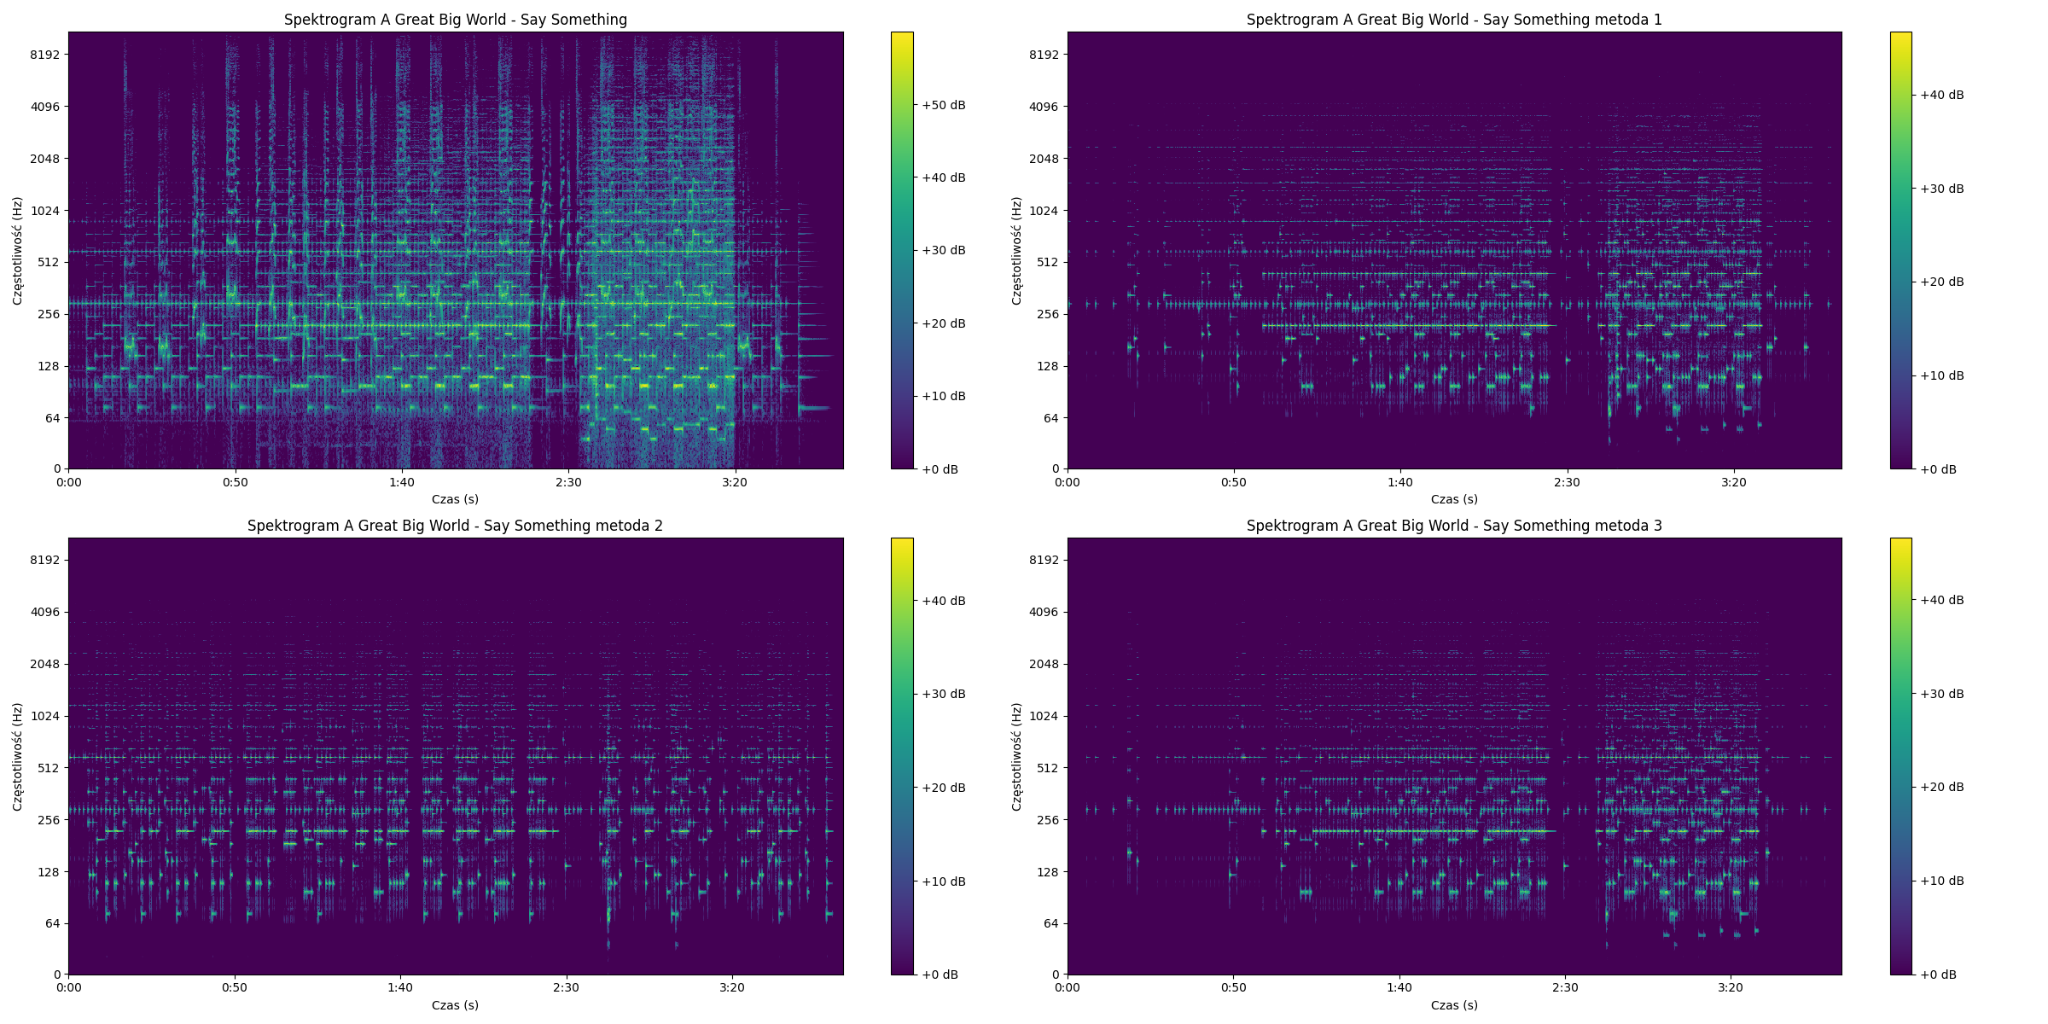
\includegraphics[width=0.82\textwidth]{img/5/wid3.png}
  \caption{Wykres przedstawiający widmo wejściowego nagrania oraz \\wyjściowych ścieżek dźwiękowych}
\end{figure}

\noindent Współczynnik m przy wartości maksymalnej użyty w pierwszej metodzie wynosił 0.76.
W drugiej metodzie współczynnik k, czyli czyli stosunku średniej wszystkich wartości w małym otoczeniu czasu do wartości maksymalnej wynosił 0.5, a dzielnik d wynosił 0.6.
W trzeciej metodzie współczynnik k, czyli stosunku średniej wartości w małym otoczeniu do wartości maksymalnej wynosił 0.3, a dzielnik d wynosił 1.1.

\newpage
\subsection{Hallelujah}

\textbf{Piosenka powstała z syntezy pliku midi}

\begin{figure}[h]
  \centering
  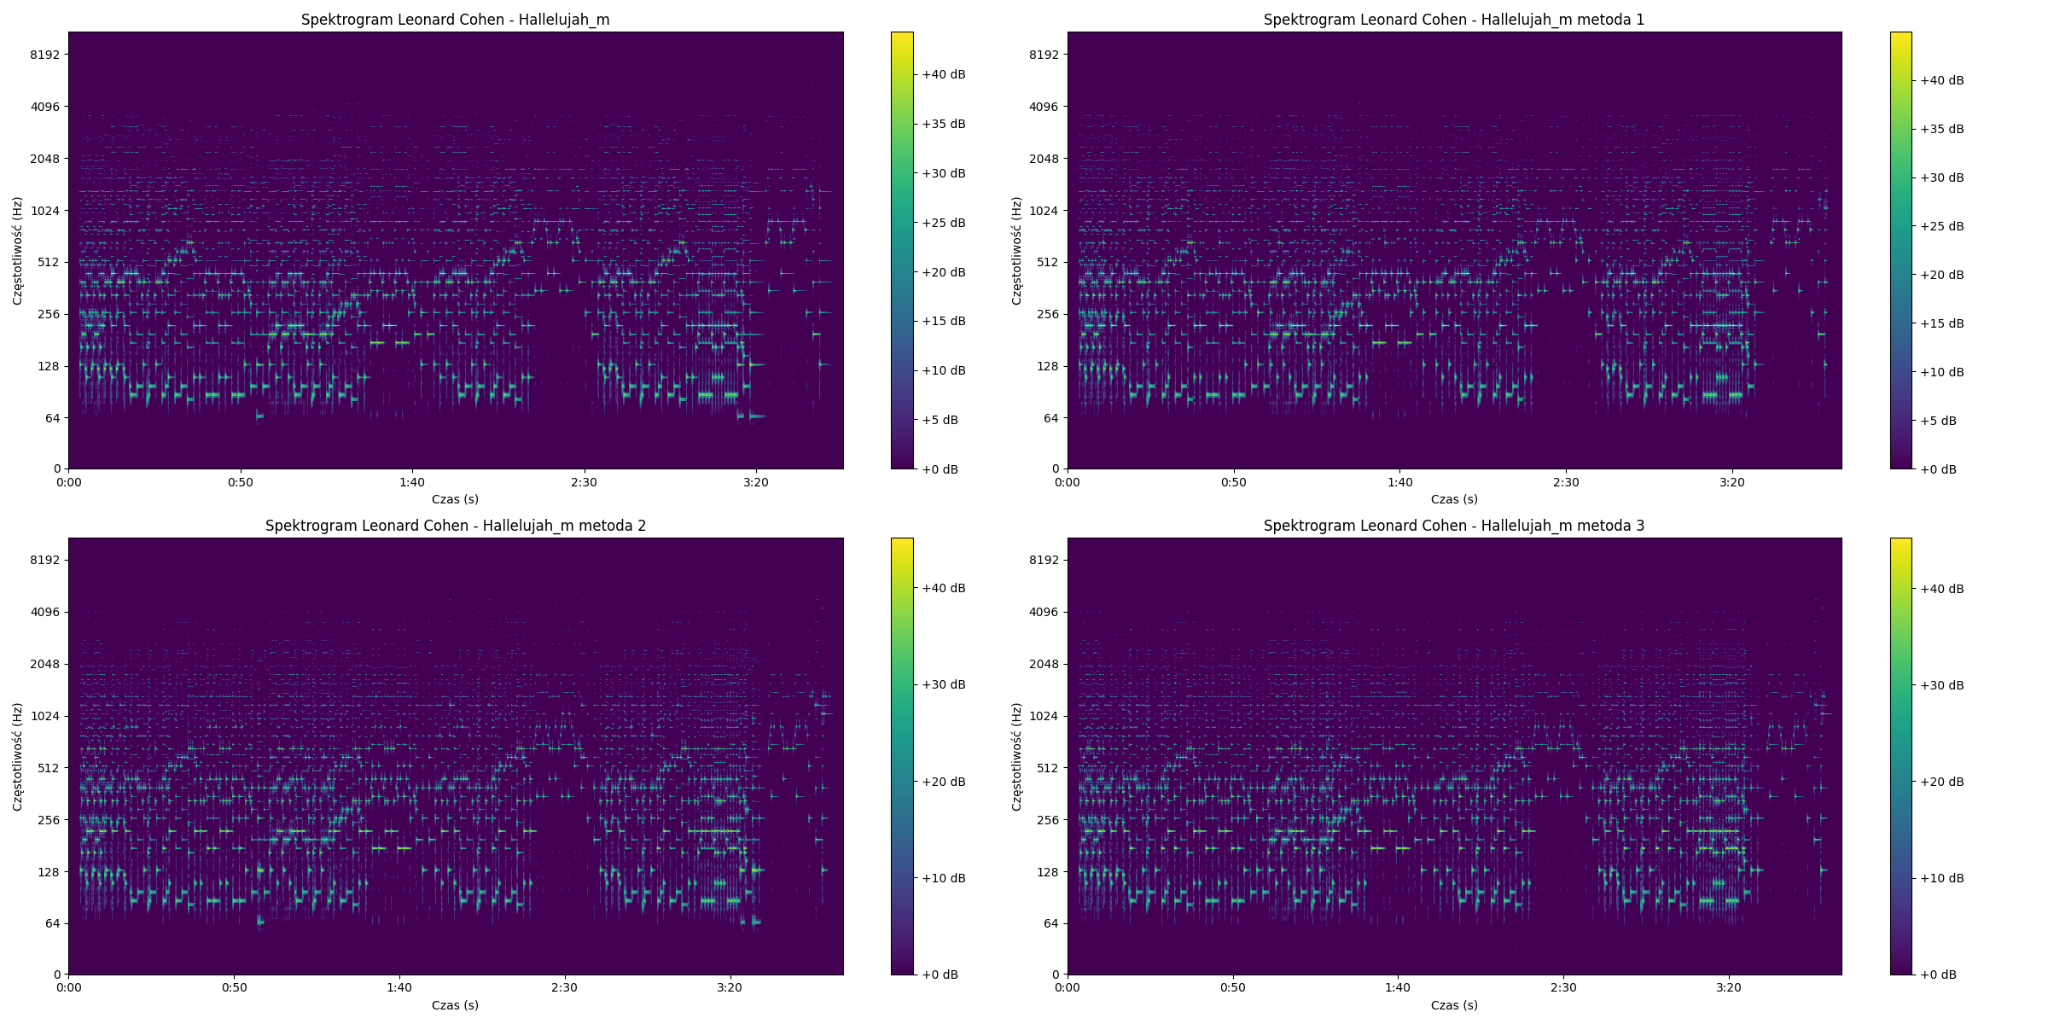
\includegraphics[width=0.82\textwidth]{img/5/wid4.png}
  \caption{Wykres przedstawiający widmo wejściowego nagrania oraz \\wyjściowych ścieżek dźwiękowych}
\end{figure}

\noindent Współczynnik m przy wartości maksymalnej użyty w pierwszej metodzie wynosił 0.66.
W drugiej metodzie współczynnik k, czyli stosunku średniej wszystkich wartości w małym otoczeniu czasu do wartości maksymalnej wynosił 0.4, a dzielnik d wynosił 0.6.
W trzeciej metodzie współczynnik k, czyli stosunku średniej wartości w małym otoczeniu do wartości maksymalnej wynosił 0.4, a dzielnik d wynosił 1.2.\\

\textbf{Piosenka zagrana na instrumencie klawiszowym typu pianino, bądź fortepian}

\begin{figure}[h]
  \centering
  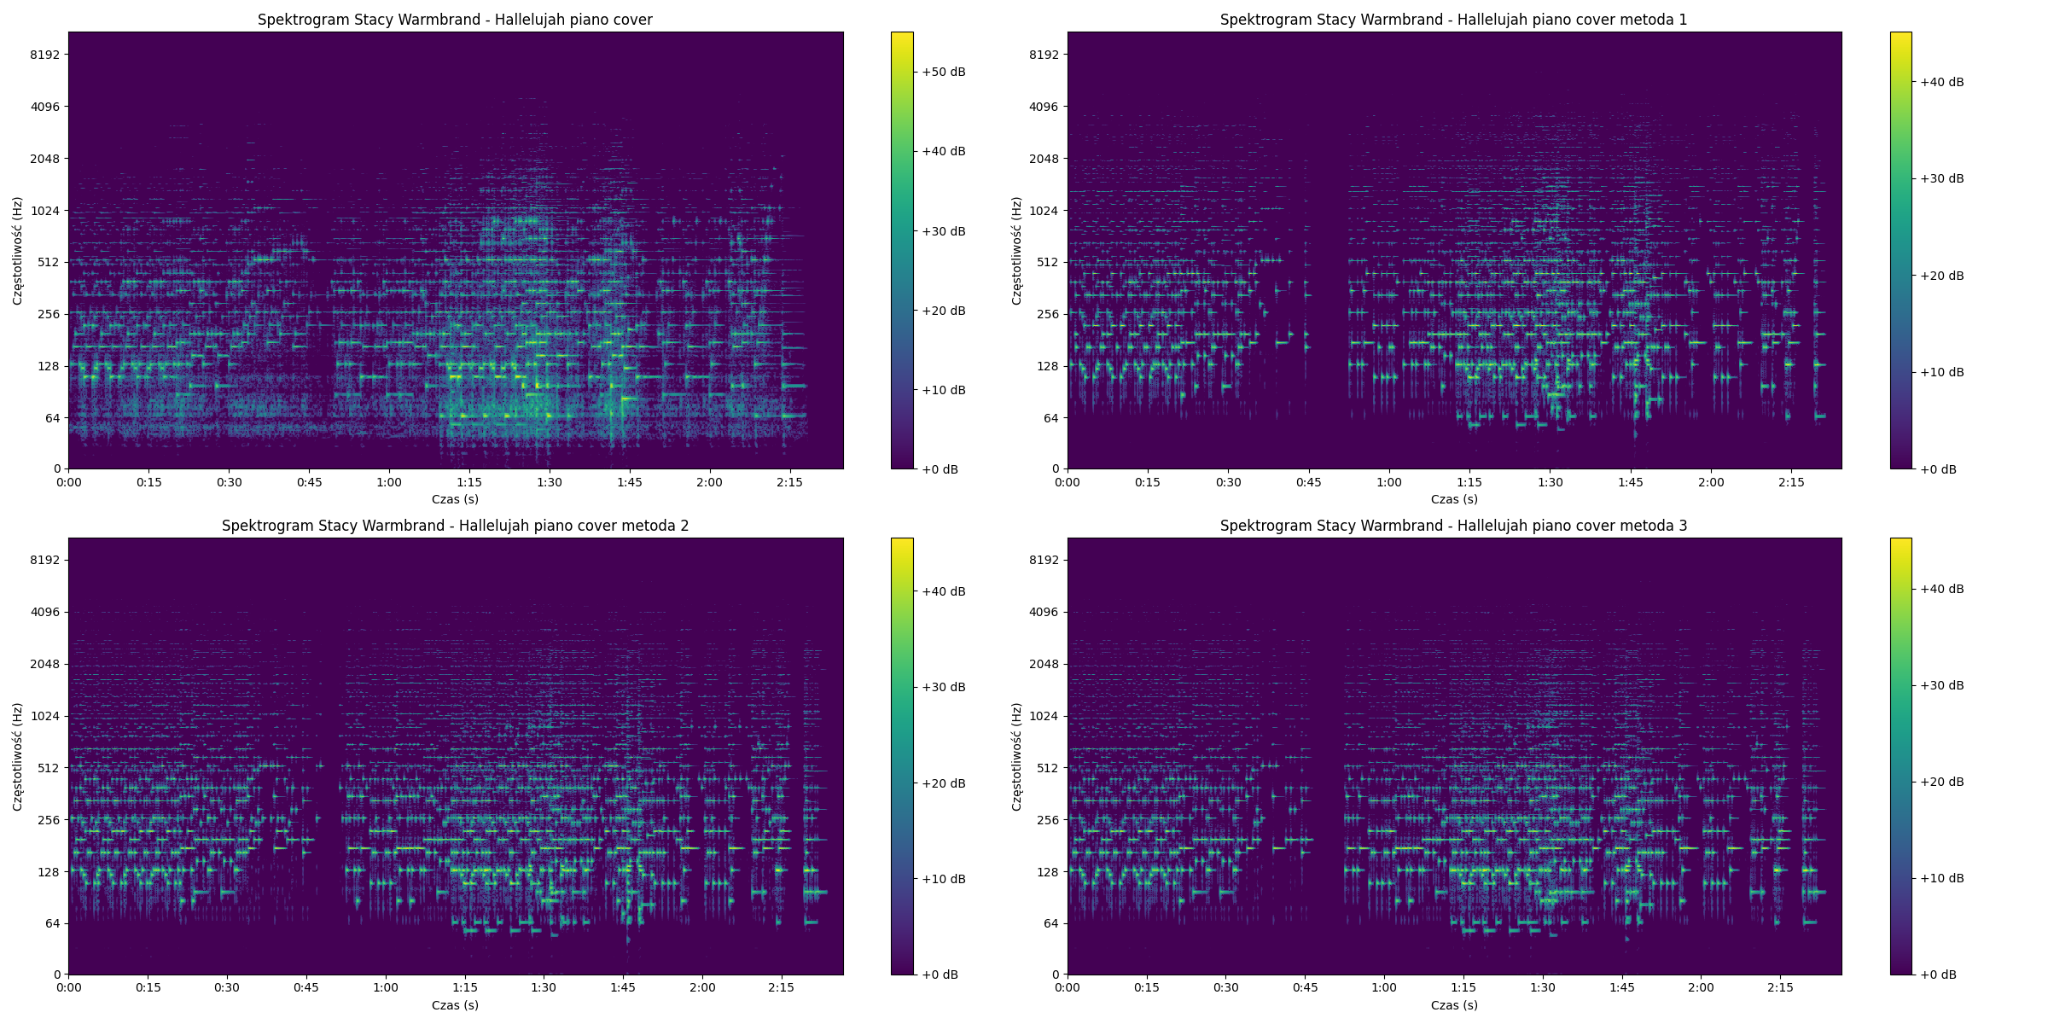
\includegraphics[width=0.82\textwidth]{img/5/wid5.png}
  \caption{Wykres przedstawiający widmo wejściowego nagrania oraz \\wyjściowych ścieżek dźwiękowych}
\end{figure}

\noindent Współczynnik m przy wartości maksymalnej użyty w pierwszej metodzie wynosił 0.64.
W drugiej metodzie współczynnik k, czyli stosunku średniej wszystkich wartości w małym otoczeniu czasu do wartości maksymalnej wynosił 0.5, a dzielnik d wynosił 0.55.
W trzeciej metodzie współczynnik k, czyli stosunku średniej wartości w małym otoczeniu do wartości maksymalnej wynosił 0.45, a dzielnik d wynosił 1.2.\\

\textbf{Oryginalna piosenka zawierająca wokal}

\begin{figure}[h]
  \centering
  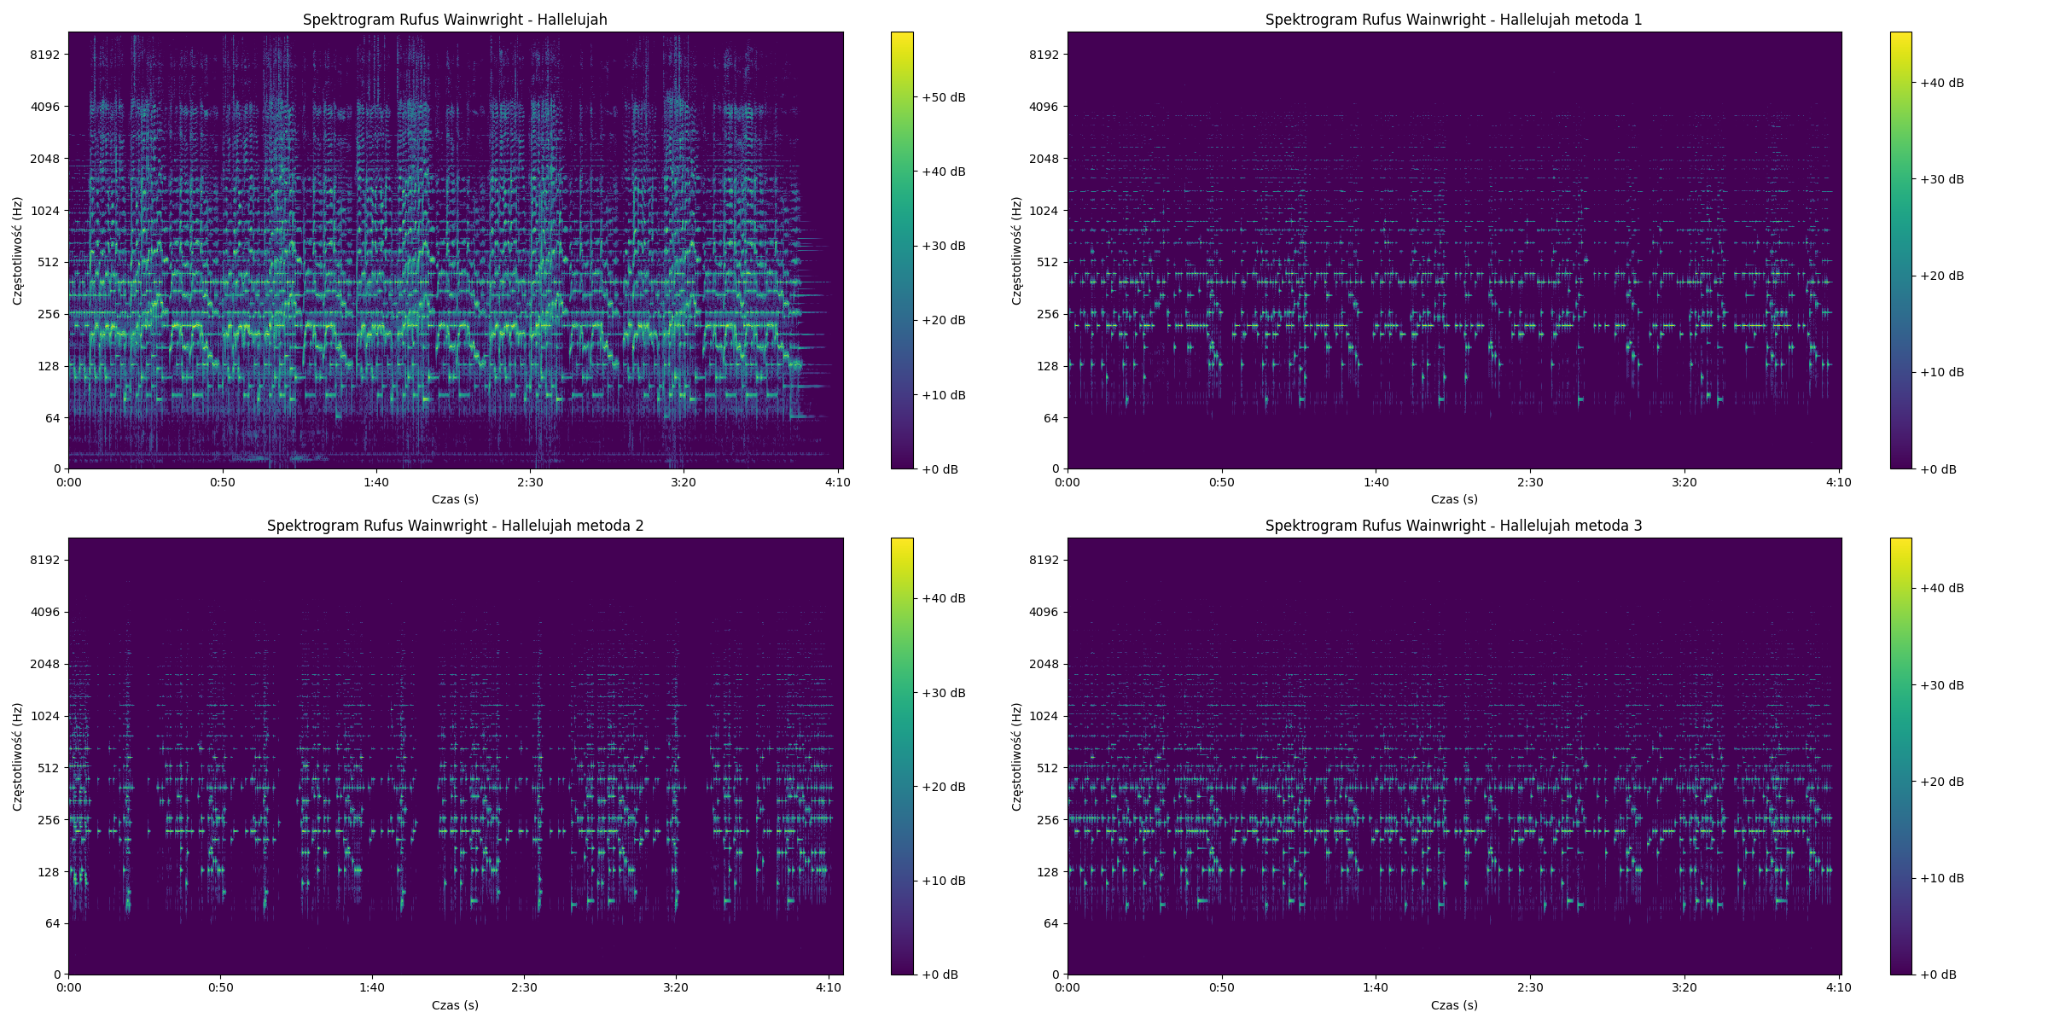
\includegraphics[width=0.82\textwidth]{img/5/wid6.png}
  \caption{Wykres przedstawiający widmo wejściowego nagrania oraz \\wyjściowych ścieżek dźwiękowych}
\end{figure}


\noindent Współczynnik m przy wartości maksymalnej użyty w pierwszej metodzie wynosił 0.79.
W drugiej metodzie współczynnik k, czyli stosunku średniej wszystkich wartości w małym otoczeniu czasu do wartości maksymalnej wynosił 0.6, a dzielnik d wynosił 0.46.
W trzeciej metodzie współczynnik k, czyli stosunku średniej wartości w małym otoczeniu do wartości maksymalnej wynosił 0.3, a dzielnik d wynosił 1.15.

\newpage
\subsection{Falling Apart}

\textbf{Piosenka powstała z syntezy pliku midi}

\begin{figure}[h]
  \centering
  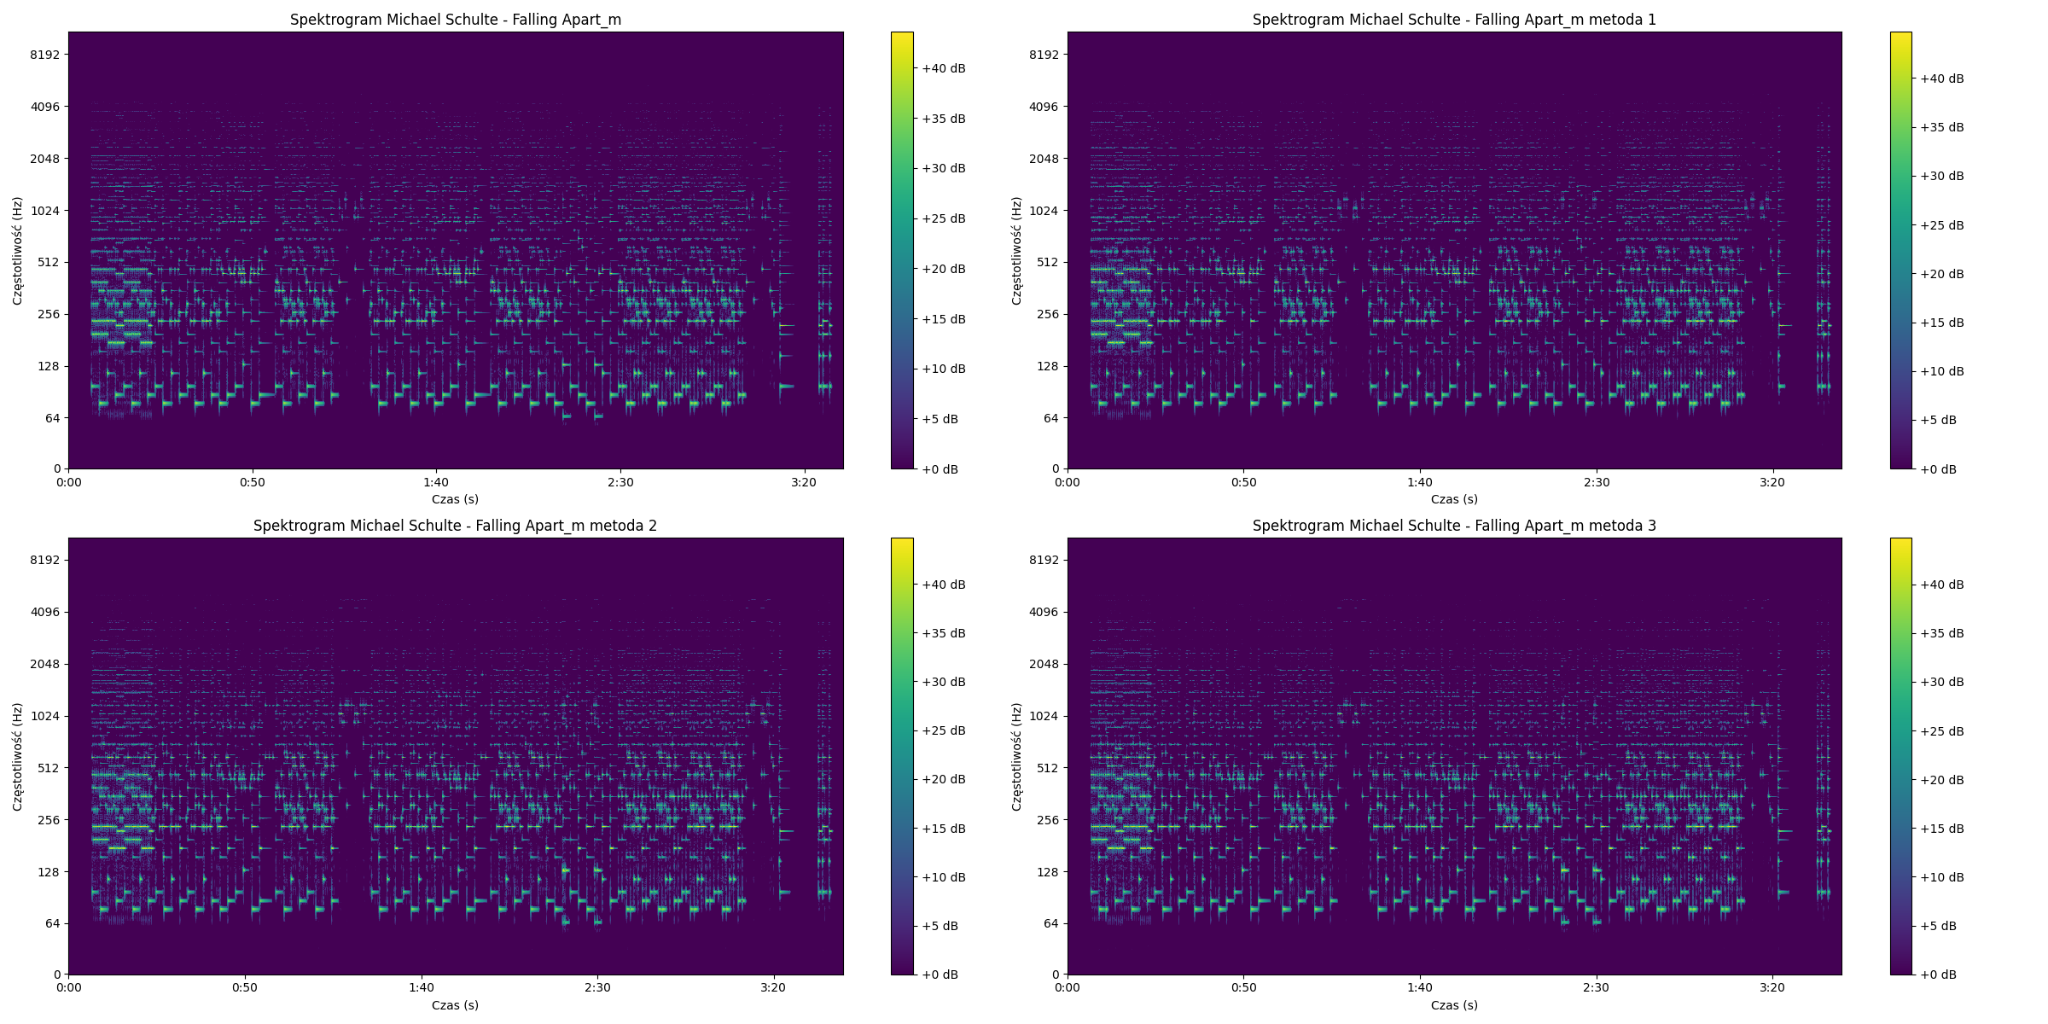
\includegraphics[width=0.82\textwidth]{img/5/wid7.png}
  \caption{Wykres przedstawiający widmo wejściowego nagrania oraz \\wyjściowych ścieżek dźwiękowych}
\end{figure}

\noindent Współczynnik m przy wartości maksymalnej użyty w pierwszej metodzie wynosił 0.66.
W drugiej metodzie współczynnik k, czyli stosunku średniej wszystkich wartości w małym otoczeniu czasu do wartości maksymalnej wynosił 0.4, a dzielnik d wynosił 0.6.
W trzeciej metodzie współczynnik k, czyli stosunku średniej wartości w małym otoczeniu do wartości maksymalnej wynosił 0.4, a dzielnik d wynosił 1.2.\\

\textbf{Piosenka zagrana na instrumencie klawiszowym typu pianino, bądź fortepian}

\begin{figure}[h]
  \centering
  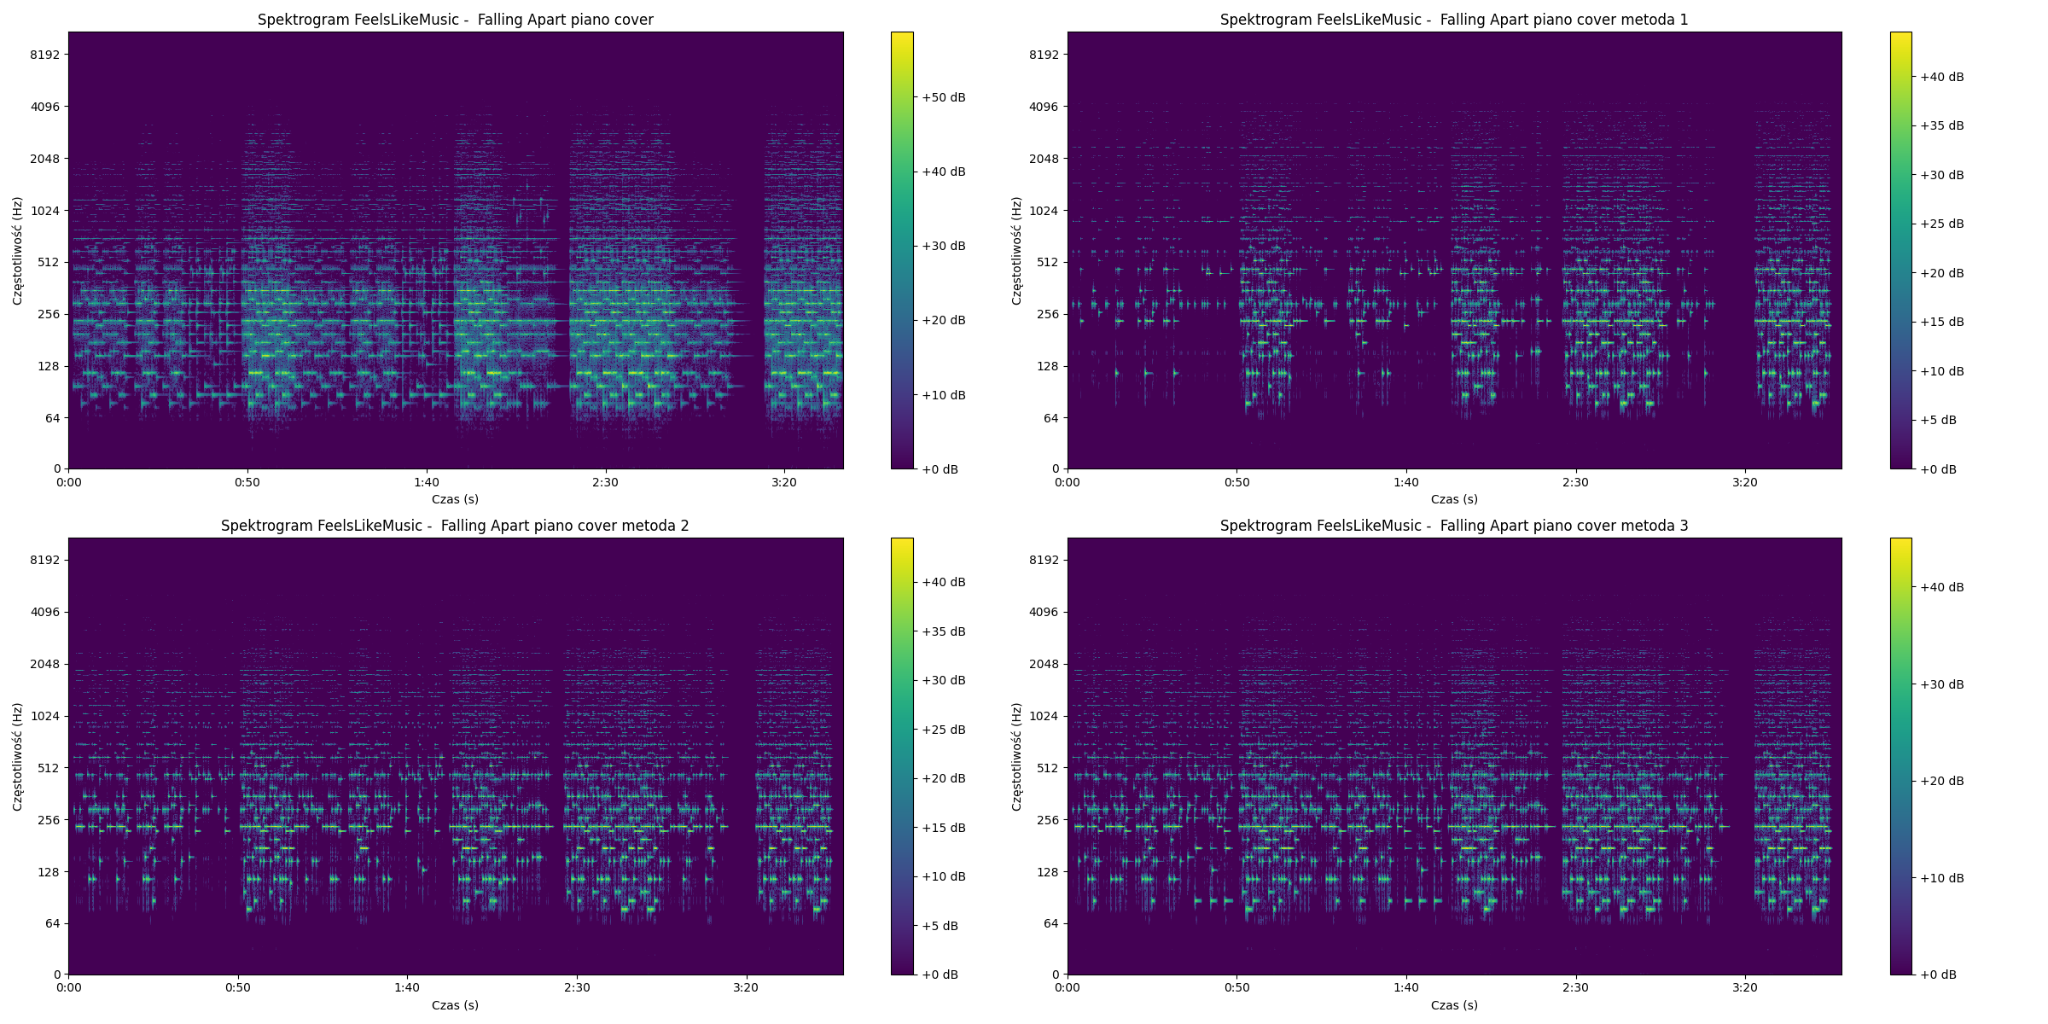
\includegraphics[width=0.82\textwidth]{img/5/wid8.png}
  \caption{Wykres przedstawiający widmo wejściowego nagrania oraz \\wyjściowych ścieżek dźwiękowych}
\end{figure}

\noindent Współczynnik m przy wartości maksymalnej użyty w pierwszej metodzie wynosił 0.71.
W drugiej metodzie współczynnik k, czyli stosunku średniej wszystkich wartości w małym otoczeniu czasu do wartości maksymalnej wynosił 0.5, a dzielnik d wynosił 0.53.
W trzeciej metodzie współczynnik k, czyli stosunku średniej wartości w małym otoczeniu do wartości maksymalnej wynosił 0.5, a dzielnik d wynosił 1.1.\\

\textbf{Oryginalna piosenka zawierająca wokal}


\begin{figure}[h]
  \centering
  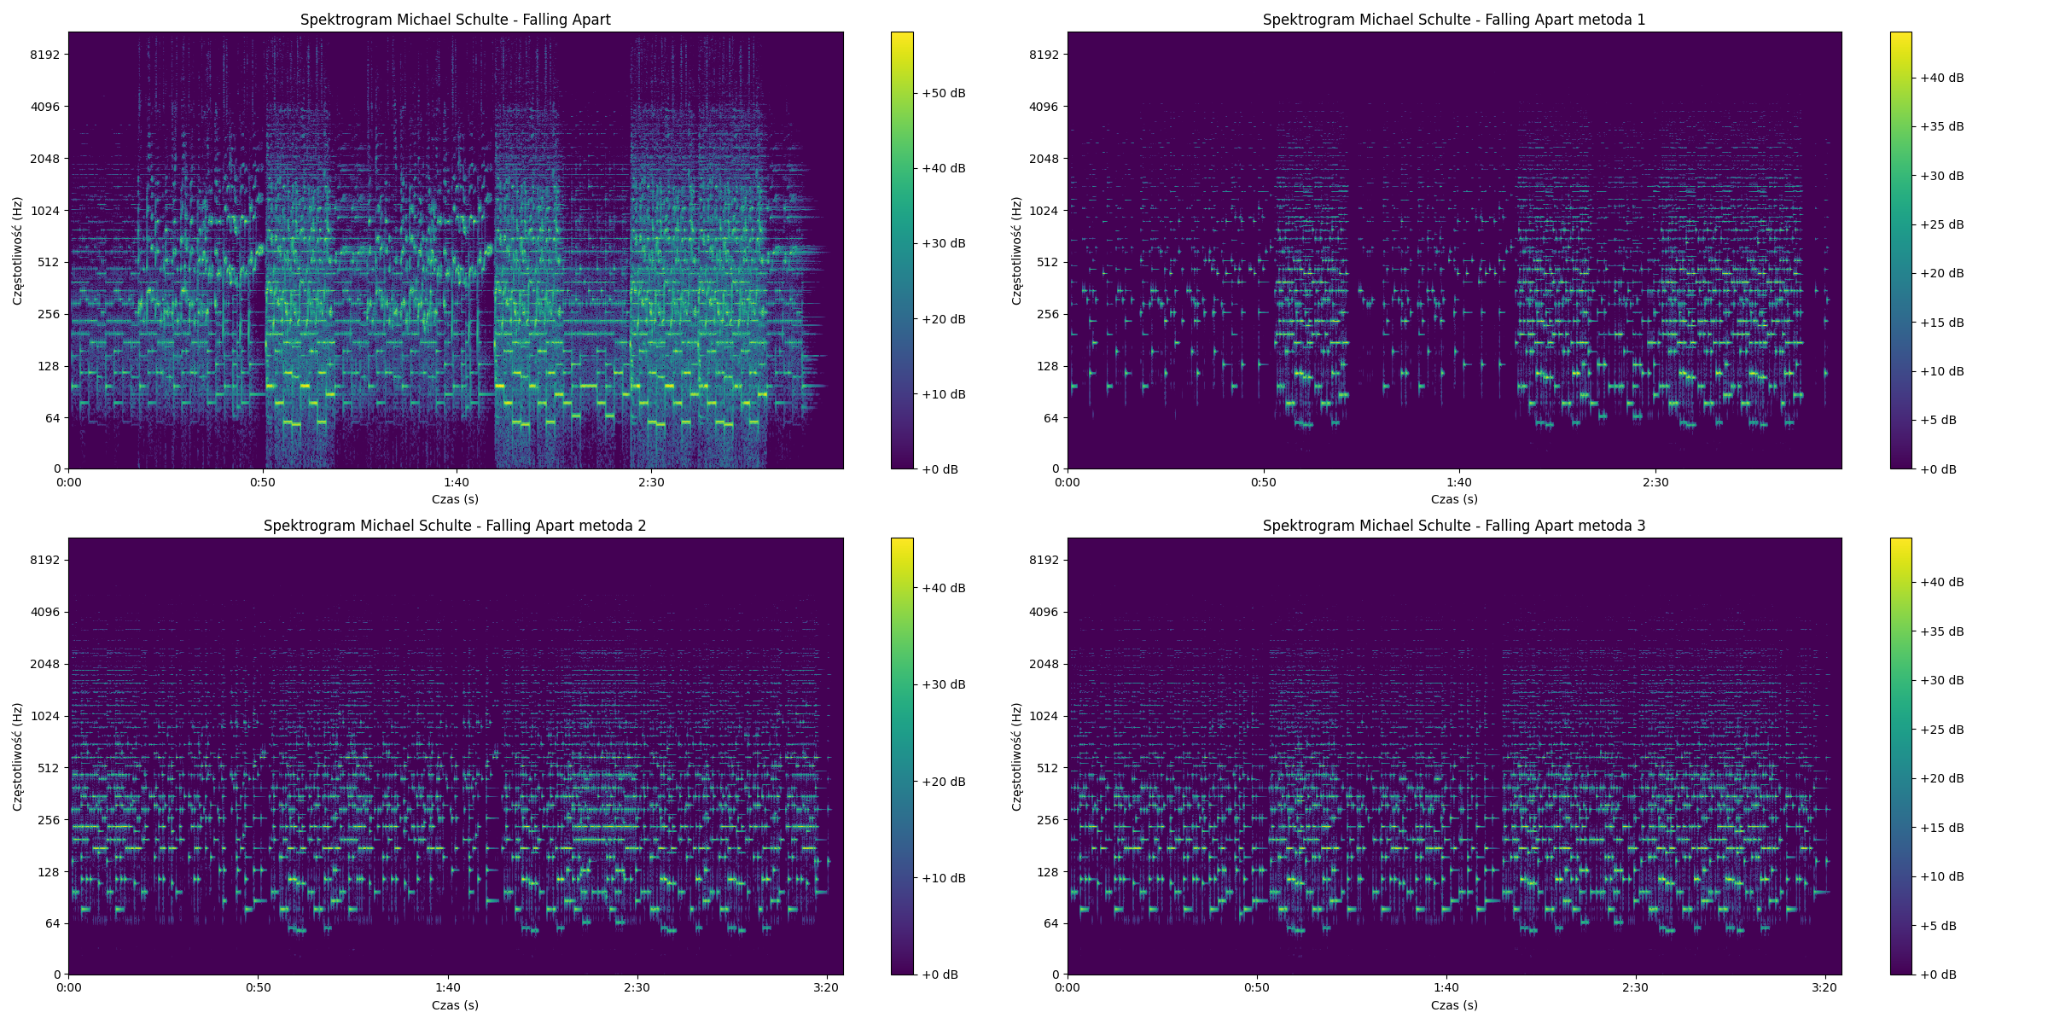
\includegraphics[width=0.82\textwidth]{img/5/wid9.png}
  \caption{Wykres przedstawiający widmo wejściowego nagrania oraz \\wyjściowych ścieżek dźwiękowych}
\end{figure}

\noindent Współczynnik m przy wartości maksymalnej użyty w pierwszej metodzie wynosił 0.75.
W drugiej metodzie współczynnik k, czyli stosunku średniej wszystkich wartości w małym otoczeniu czasu do wartości maksymalnej wynosił 0.6, a dzielnik d wynosił 0.46.
W trzeciej metodzie współczynnik k, czyli stosunku średniej wartości w małym otoczeniu do wartości maksymalnej wynosił 0.6, a dzielnik d wynosił 1.

\subsection{Wyświetlanie synthesii}

Wszystkie wskazówki graficzne są poprawnie wyświetlane ze względu na ton. We fragmentach, w których naciskane jest więcej klawiszy w jednym momencie, program ze względu na swoją prędkość działania powoduje opóźnienie w pojawieniu się każdego klawisza, przez co powstaje niewielkie przesunięcie względem siebie. Natomiast ze względu na potrzebę użycia akumulatora, który kompensuje opóźnienia zależne od ilości wyświetlanych elementów, potrafi nie zgadzać się ich długość. Spowodowane jest to wpływem zmiennej prędkości wyświetlania na długość trwania każdego tonu.

\section{Analiza i ocena poprawności odtwarzania tonów}

Wyjściowa sekwencja muzyczna wybrzmiewała identycznie dla wejściowej syntetycznie wygenerowanej piosenki. Każda z metod świetnie się sprawuje przy tak stworzonym dźwięku. Powodem tego jest praktycznie stały poziom amplitudy dla wszystkich głównych dźwięków oraz dobra identyfikacja dźwięków harmonicznych, które zwykle rozpoczynają się równo z dźwiękiem, z którego powstały, dzięki czemu niewiele z nich wybrzmiewa w wynikowej sekwencji.

Utwór muzyczny grany na pianinie przyniósł znacznie słabszą jakość detekcji. Pierwsza metoda, gdzie parametr graniczny był stały nie radził sobie z amplitudą zmieniającą się wraz z każdym pojedynczym dźwiękiem. W ten sposób powstały miejsca wyciszenia, gdzie nie został żaden dźwięk wyłapany, bądź pojedyncze oraz miejsca zgłośnień, gdzie zmiana dynamiki gry na bardziej eksplozywną powodowała wyłapanie wielu składowych harmonicznych, które potrafiły kompletnie zniekształcić piosenkę. Dużo lepiej tutaj radziła sobie metoda druga, która zmieniała parametr detekcji wraz z czasem piosenki, przez co zmienna dynamika nie stanowiła już takiego problemu, jak przy użyciu poprzedniej metody. Jednakże wynik zauważalnie odbiega od wyniku przy syntezowanej piosence. Spowodowane jest to bogactwem i głębią dźwięku, co za tym idzie, złożeniem składowych harmonicznych, które bardzo utrudniają analizę utworu. Trzecia metoda, radziła sobie podobnie do drugiej metody, momentami znajdując więcej poprawnych tonów, niemniej jednak kosztem przechwytywania większej ilości dźwięków harmonicznych. Powodem tego jest dobieranie progu ze względu na najbliższe otoczenie, co pomaga znaleźć wśród reszty tony o niższej amplitudzie, jak i zarazem składowe harmoniczne, które nie 
odznaczały się tak bardzo głośnością, aby zostać wykryte przez poprzednie algorytmy.

Analiza oryginalnego utworu muzycznego przyniosła podobne efekty co utworu granego na pianinie z mniejszą dokładnością. Pierwsza metoda nie poradziła sobie ze zmiennością amplitudy w czasie, co przełożyło się na miejsca z widocznymi dziurami oraz miejsca przesilenia ilości wykrytych tonów. Druga metoda radziła sobie gorzej niż w poprzednim typie utworu muzycznego. Zmienność progu detekcji zależnej od czasu, nie radził sobie ze zmiennością amplitudy pomiędzy wokalem a instrumentami, co powodowało częste luki w detekcji śpiewu. Trzecia metoda poradziła sobie z oryginalnym utworem podobnie do wersji odtworzonej na pianinie. Różnica w amplitudach wokalu i instrumentów nie była tak znacząca, dzięki zmienności progu detekcji w zależności od najbliższego otoczenia, co niestety wciąż przekłada się na wrażliwość tej metody na dźwięki harmoniczne o niższej amplitudzie, które nie były wykrywane przez pozostałe metody.

Detekcja czasu rozpoczęcia się danego dźwięku, w każdym scenariuszu testowym była na wysokim poziomie. Wyszukiwanie maksimum lokalnego i cofanie się do kolejnego punktu przegięcia pozwalało rozpocząć dźwięk równo z zauważeniem wzrostu amplitudy przez jego zagranie. Tylko w nielicznych momentach mogło zostać to zagłuszone przez główne tony lub dźwięki harmoniczne o bardzo bliskiej częstotliwości. Detekcja czasu trwania dźwięku jest poprawna, jednak mało dokładna. Powodem jest stały próg zakończenia trwania dźwięku. Nie mógł zostać zdefiniowany jako znalezienie minimum lokalnego, którym rzeczywiście charakteryzuje się zakończony dźwięk, ponieważ w czasie jego trwania, pozostałe tony, które odznaczają się składowymi harmonicznymi na podobnej częstotliwości, mogłyby powodować znacząco przedwczesne zakończenie się trwania tonu.

\section{Problemy i ograniczenia napotkane podczas implementacji}

Jednym z najtrudniejszych problemów okazała się zmienność amplitudy w piosence, co wymagało zaimplementowania bardziej skomplikowanych metod detekcji. Trudność ta spowodowała również niedokładność przy przeplataniu się dwóch instrumentów, bądź ich składowych harmonicznych, co powodowało brak wykrywalności wielu tonów, które zostawały przykryte przez silniejszy sygnał.
Barierą nie do pokonania w pełni okazały się składowe harmoniczne, które jak wcześniej zostało wspomniane niejednokrotnie odznaczały się jako główne dźwięki, których nie sposób jednoznacznie zidentyfikować.
